\section{\edpsgui: the \edps\ dashboard}


To launch the \edps\ dashboard, type:
\begin{verbatim}
  . <path-to-environment>/bin/activate 
  edps-gui
\end{verbatim}
The {\tt <path-to-environment>} is the full-path-name of the virtual
environment defined during the installation procedure.

The \edpsgui\ is then loaded on a browser window (see Figure
\ref{fig:gui}). To start \edps, press the {\tt Start EDPS} green
button at the top of the window. To stop \edps, press the {\tt Stop
  EDPS} red button and press `Ctrl-c` on the terminal where the
\edpsgui\ command was launched.



\begin{figure}[h!]
\centering
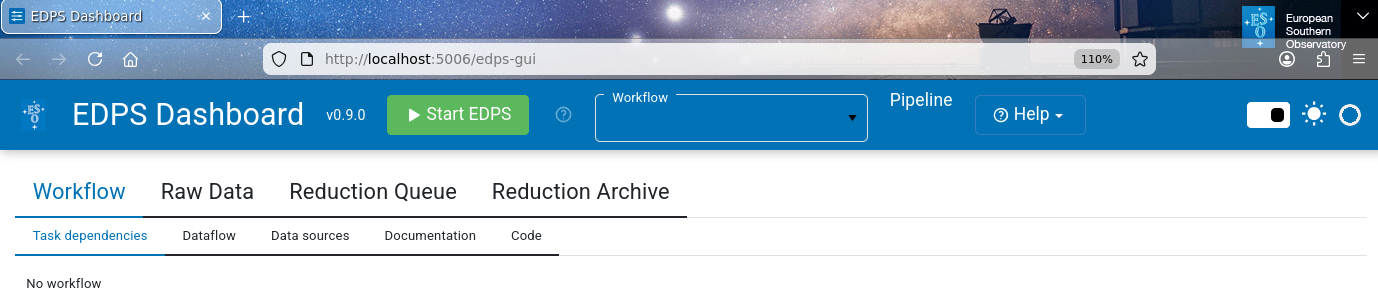
\includegraphics[width=0.9\textwidth]{figures/gui.jpg}
\caption{The \edpsgui\ dashboard (Graphic User Interface). At this stage, \edps\
has not been started yet and no workflow has been selected.}
\label{fig:gui}
\end{figure}

At the top of the Dashboard, near the {\tt Start/Stop EDPS} buttons there
is the {\bf Workflow} selection menu, which allows to load the desired
workflow. The available workflows depend on the pipelines installed in
your system.

The {\tt Help} drop-down menu contains version information, reference,
and the {\bf Settings} menu, which allows to configure several
\edps\ behaviours, such as links to data-storage directories, and the
parallelization.  It is described in detail in Section
\ref{sec:settings}. Note that it is possible to change the
settings only if \edps\ has not been started yet.

There are 4 tabs in the main dashboard window, they are:

\begin{itemize}
\item {\bf Workflow}. It gives information on the workflow, the graphic
  layout, a description of the type of data and access to the workflow
  code. It is described in detail in Section \ref{sec:workflow_tab}.


\item {\bf Raw Data}. It allows to specify the input data, the preferences
  for association calibrations, and to create datasets to be reduced. It
  is described in Section \ref{sec:raw_data_tab}.


\item {\bf Reduction Queue}. It starts the data reduction. It is described in
  Section \ref{sec:reduction_queue_tab}.


\item {\bf Reduction Archive}. It gives access to previously archived data
  reduction and final products. It is described in Section \ref{sec:reduction_archive_tab}.
  
\end{itemize}

At the bottom of the dashboard, the graphic representation of the
selected workflow is visible (e.g. Figure \ref{fig:workflow_tab}).


\subsection{Settings}
\label{sec:settings}

Several options in \edps\ can be specified in a configuration file, named {\tt application.properties}.
This file is located in the {\tt .edps/} directory in your {\tt HOME} directory.  It is possible to modify the file directly through the EDPS-GUI, by selecting the menu "Settings" in the drop-down menu "Help" at the top of the GUI (Figure \ref{fig:help_settings}). 


\begin{figure}[h!]
\centering
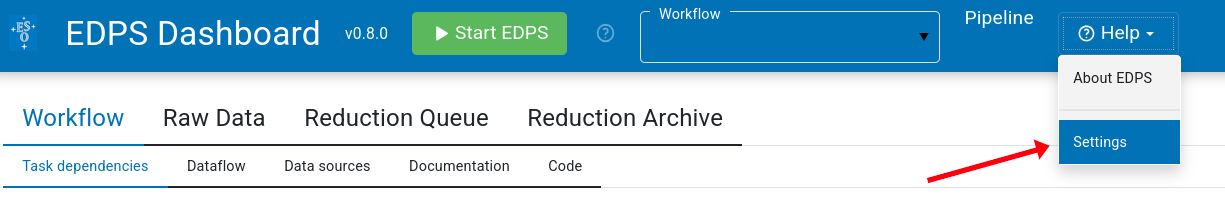
\includegraphics[width=0.9\textwidth]{../common/figures/help_settings.jpg}
\caption{Location of the "Settings" menu. Settings have to be changed while \edps\ is not running.}
\label{fig:help_settings}
\end{figure}


Note, the file can be edited only if \edps\ is not running; press the {\tt Stop EDPS} red button if necessary.
In the following, we describe the most important configuration variables. After the settings are changed, press the {\tt SAVE} button to save.
They new values will be used when pressing {\tt Start EDPS} the next time.

\begin{itemize}
\item {\bf Location of products and database}: The {\tt base\_dir}  and {\tt path} variables.

  This is the folder where \edps\ saves all the products of all the executed jobs (specified via  {\tt base\_dir}), as well as it keeps a database with the information of the various reductions (specified via {\tt path}). These are specified at the first execution of the \edpsgui, but
  it might be convenient to change it, e.g. if the selected location has no more space.
  Obviously, if new values are specified, all the information stored in the previous location is no longer visible.
  It is recommended to specify full paths, otherwise a new directory will be created every time on the path the \edpsgui\ is launched from.

\item {\bf Association preference}: RAW vs MASTER calibrations.
\label{list:association_preferences}

   {\it Note: it is recommended to specify this variable via the GUI, before 
   creating the datasets (see Section \ref{sec:raw_data_tab})   
   and not by editing the {\tt application.properties} file.}
 
   If the input directory contain both MASTER (e.g., pre-reduced calibrations) and RAW calibrations, it could happen that both of them fulfil the matching criteria and quality level for a certain task. In this case, one can specify to which type of calibration to give priority by setting the variable {\tt association\_preference} in the  configuration file.  Possible values of {\tt association\_preference} are:
   
   \begin{itemize}
    \item  {\bf raw}. First, EDPS checks if there are raw calibrations ensuring the first quality level of the products (see Section \ref{sec:association_levels}). If found, they are associated. If not found, raw calibrations ensuring the second quality
    level of the products are searched. If not found, the next level is searched until the last quality level  is reached.
    If no raw calibrations are found for none of the quality levels, then EDPS searches for master calibrations, starting from those ensuring the first quality level. If none are found, the second
    level is searched, and so forth. If no calibrations are found, the association is not done.
    
   \item {\bf master}. Same as raw, but first master calibrations are looked for all the products quality levels permitted by the workflow parameter {\tt quality\_threshold}. Then, if master calibrations are not found, the system looks for raw calibrations.
   
    \item {\bf raw\_per\_quality\_level} (default). First, the system will check if there are raw calibrations ensuring the first quality level of the products. If not found, MASTER calibrations ensuring this level are searched for. If not found, RAW calibrations ensuring the second quality
     level are searched for, if not found MASTER calibrations matching the second quality level are
     searched for. The sequence goes on until the last level permitted by the workflow parameter quality\_threshold.
     
  \item {\bf master\_per\_quality\_level}. Same as raw\_per\_quality\_level, but with inverted roles
     for MASTER and RAW calibrations.
     If a combination of RAW and MASTER calibrations are present, the value of association\_preference
     might have an impact on the performances and the quality of the results. Typically. association\_
     preference = raw\_per\_quality\_level delivers the best quality products, at the price of speed. 
    On the other hand, association\_preference = master ensures faster performances, at cost
   of quality (e.g., a very old master calibration could be used instead a more recent raw calibration). If
   only RAW or MASTER calibrations are present in the input directories, then the value of association\_preference has no impact.
\end{itemize}

\item {\bf Parallelization}
   One of the advantages of \edps\ is that it can exploit powerful hardware. The following variables in
  the {\tt application.properties} file determine the parallelization of EDPS reduction.
  \begin{itemize}
  \item {\bf processes} (default: 1). It specifies the maximum number of jobs to run in parallel (e.g. \esorex\ parallel executions).
  \item {\bf cores} (default: 1). It specifies the maximum numbers of computers cores to use, considering
all the parallel jobs.

  \item {\bf default\_omp\_threads} (default: 1). The number of cores to use for each job. This can be overridden by specifying a recipe parameter {\tt OMP\_NUM\_THREAD} for a given task when configuring the reduction.
  
\end{itemize}

  The optimal configuration depends on the system and on the instrument pipeline (e.g., whether it is parallelized or not).
  
  In case of parallelized pipelines,  we recommend to reserve to \edps\ the full number of cores (minus 1). Set 2 processes in parallel, 
  and default\_omp\_threads to about 1/2 of cores.

  In case of non parallelized pipelines, we recommend to  reserve to \edps\ the full number of cores (minus 1). Set the number of parallel processes as the number of allocated cores, and
  default\_omp\_threads to 1.


\item {\bf Order of executions}.
The variable ordering in the {\tt application.properties} file specifies the priority to give to the
reduction jobs. The most important values are:
\begin{itemize}
  \item {\bf dfs}. depth-first, gives preference to reaching final reduction target quicker. In other words, it
finish the reduction of a dataset before moving to the next dataset. This choice is less efficient
in time but it gives priority to the reduction of individual datasets.
  \item {\bf type}. It gives preference to following the reduction cascade level by level making sure to process same type of data together (eg. first all biases).
  \item {\bf dynamic}. Immediately runs whichever job is ready (has all needed inputs), no stalling but the
order is unpredictable. This is the most time efficient execution order.

\end{itemize}

\end{itemize}
